\section{LLVM}




\subsubsection{PGO and LLVM}

Profile Guided Optimizations.

\subsection{Profile Guided Transforms}

\subsubsection{Spill Placement}
registers

\subsubsection{Code Layout}

Code layout \cite{raman2022learning} is the process of ordering the blocks of the CFG. This order dictates the
placement of instructions within those blocks in memory. By inserting branch instructions at the end of the basic blocks,
the compiler can layout the blocks in any order.  Consider the
Control Flow Graph (CFG) in Figure \ref{fig:p7}. Figures \ref{fig:p8} and \ref{fig:p9}
show two possible layouts of the CFG. In both theese layouts,
a block is followed by one of its successor blocks that is
not yet laid out. Consider block A, for example. It has two
successors in the CFG. Only one of the successors B or C 
can be placed immediately following A and is known as the
\textbf{fall-through block}. In Figure \ref{fig:p8}, B is the fall-through block
and in the layout in Figure \ref{fig:p9}, C is the fall-through block.
The choice of which block to place as the fall-through block
has performance implications. If control is often transferred
to C from A often during program execution, then placing
C next to A has the following advantages:


\begin{figure}[!htb]
    \minipage{0.5\textwidth}
      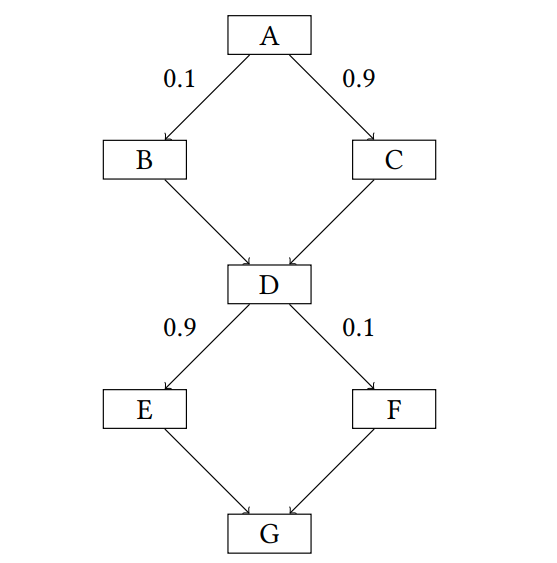
\includegraphics[width=\linewidth]{p7.png}
      \caption{CFG}\label{fig:p7}
    \endminipage\hfill
    \minipage{0.25\textwidth}
      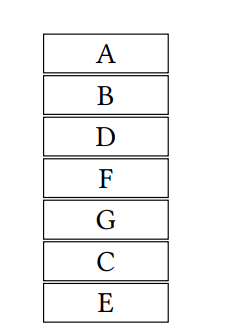
\includegraphics[width=\linewidth]{p8.png}
      \caption{Layout 1}\label{fig:p8}
    \endminipage\hfill
    \minipage{0.25\textwidth}
      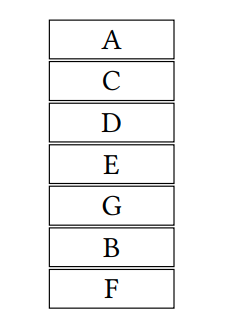
\includegraphics[width=\linewidth]{p9.png}
      \caption{Layout 2}\label{fig:p9}
    \endminipage\hfill
    \caption{Code Layout}
\end{figure}




\begin{itemize}
\item Since the branch at the end of A is mostly not-taken,
the frontend of the processor's pipeline is less likely to
be stalled if it is an out-of-order superscalar processor.
\item As the cacheline containing the last instruction of A
also contains instructions that are more likely to execute (from block C), instruction cache utilization is
likely to be better.
\end{itemize}

In the LLVM compiler, the \texttt{MachineBlockPlacement} pass
performs code layout optimization. This pass relies on the
branch probability analysis which provides, for each branch
instruction, the probability of the branch being taken.
\texttt{MachineBlockPlacement} is just one of the many transformation passes that make use of branch probability analysis.
Branch probability analysis is used in another analysis called
block frequency analysis that provides relative frequencies of
basic blocks within a function. Block frequency analysis is
used by optimizations such as inlining, spill-code placement 
in register allocation among others.

\subsubsection{Hot/Cold Partitioning}

\begin{figure}[!htb]
    \minipage{0.33\textwidth}
      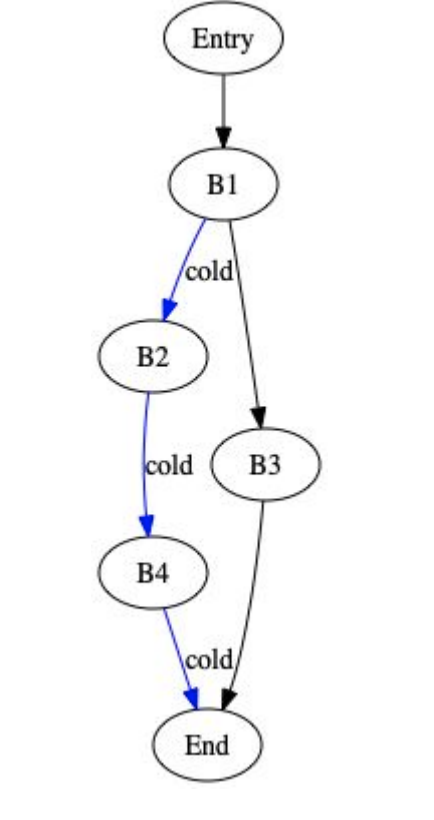
\includegraphics[width=\linewidth]{p10.png}
      \caption{CFG}\label{fig:p10}
    \endminipage\hfill
    \minipage{0.33\textwidth}
      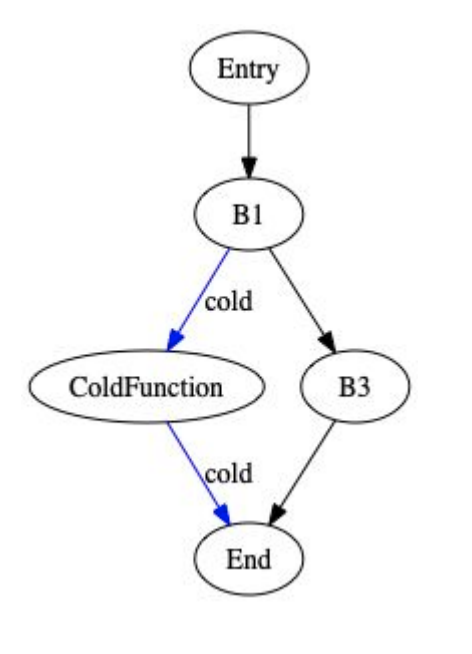
\includegraphics[width=\linewidth]{p11.png}
      \caption{Layout 1}\label{fig:p11}
    \endminipage\hfill
    \minipage{0.33\textwidth}
      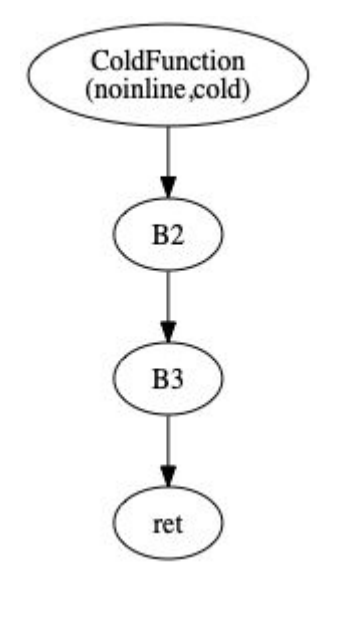
\includegraphics[width=\linewidth]{p12.png}
      \caption{Layout 2}\label{fig:p12}
    \endminipage\hfill
    \caption{Code Layout}
\end{figure}


Hot Cold splitting is an optimization to improve instruction locality. It is used to outline basic blocks which execute less frequently. The hot/cold splitting pass identifies cold basic blocks and moves them into separate functions. The linker can then put newly-created cold functions away from the rest of the program . The idea here is to have these cold pages faulted in relatively infrequently, and to improve the memory locality of code outside of the cold area.

The algorithm is novel in the sense it is based on region and implemented at the IR level. Because it is implemented at the IR level, all the backend targets benefit from this implementation. Other implementations of hot-cold splitting outline each basic block separately and are implemented at the RTL level.


What applications will benefit from Hot/Cold Spliting?

\begin{itemize}

\item High cache misses(A giant app on a small device)
\item High start-up time

\end{itemize}


\subsubsection{Inliner}



\subsubsection{Outlining \& Merging}

With PGO information, we can do more aggressive outlining of cold regions in the inline candidate function. This contrasts with the scheme of keeping only the 'early return' portion of the inline candidate and outlining the rest of the function as a single function call.

Support for outlining multiple regions of each function is added, as well as some basic heuristics to determine which regions are good to outline. Outline candidates limited to regions that are single-entry \& single-exit. Also we don't account for live-ranges we may be killing across the region with a function. These are enhancements we can consider in another patch.

Fallback to the regular partial inlining scheme is retained when either i) no regions are identified for outlining in the function, or ii) the outlined function could not be inlined in any of its callers.

\subsubsection{Control height reduction}

Control height reduction merges conditional blocks of code and reduces the
number of conditional branches in the hot path based on profiles.

\begin{lstlisting}[language=C,frame=single, caption=An ,label = lst:expr2]
  if (hot_cond1) { // Likely true.

  do_stg_hot1();
  }
  if (hot_cond2) { // Likely true.
  
  do_stg_hot2();
  }
\end{lstlisting}


\begin{lstlisting}[language=C,frame=single, caption=An ,label = lst:expr2]
  if (hot_cond1 && hot_cond2) { // Hot path.

  do_stg_hot1();
  do_stg_hot2();
  } else { // Cold path.
  
  if (hot_cond1) {
    do_stg_hot1();
  }
  if (hot_cond2) {
    do_stg_hot2();
  }
  }
\end{lstlisting}

This speeds up some internal benchmarks up to ~30\%.

\subsection{Loop Unrolling \& Loop Vectorization}


\begin{lstlisting}[language=C,frame=single, caption=An ,label = lst:expr2]
  for (int i=0; i<16; ++i)
  C[i] = A[i] + B[i];
\end{lstlisting}


\begin{lstlisting}[language=C,frame=single, caption=An ,label = lst:expr2]
  for (int i=0; i<16; i+=4) {
    C[i] = A[i] + B[i];
    C[i+1] = A[i+1] + B[i+1];
    C[i+2] = A[i+2] + B[i+2];
    C[i+3] = A[i+3] + B[i+3];
    }
\end{lstlisting}

\begin{lstlisting}[language=C,frame=single, caption=An ,label = lst:expr2]
  for (int i=0; i<16; i+=4)
  addFourThingsAtOnceAndStoreResult(
  &C[i], &A[i], &B[i]);
\end{lstlisting}
\subsection{Partial Inline}

\begin{lstlisting}[language=C,frame=single, caption=An ,label = lst:expr2]
  for (int i=0; i<16; i+=4)
  addFourThingsAtOnceAndStoreResult(
  &C[i], &A[i], &B[i]);
\end{lstlisting}

\subsection{Partial Inline }

\begin{lstlisting}[language=C,frame=single, caption=An ,label = lst:expr2]
  void foo() {
    bar();
    // rest of the code in foo
    }
    void bar() {
    if (X)
    return;
    // rest of code (to be outlined)
    }
\end{lstlisting}


\begin{lstlisting}[language=C,frame=single, caption=An ,label = lst:expr2]
  void foo() {
    if (!X)
    bar.outlined();
    // rest of the code in foo
    }
    void bar.outlined() {
    // rest of the code in bar
    }
\end{lstlisting}